\section{Redes Neurais Convolucionais (CNNs)}
\subsection{Introdução ao Conceito}
\textbf{}  
\setcounter{figure}{0}

\textbf{Definição:}  
Redes Neurais Convolucionais (CNNs) são uma classe de modelos de aprendizado profundo projetadas para processar dados estruturados em forma de grade, como imagens e séries temporais. Elas utilizam camadas convolucionais para extrair automaticamente características hierárquicas dos dados, reduzindo a complexidade computacional e melhorando a eficiência do treinamento.

\textbf{Contextualização:}  
As CNNs revolucionaram o campo da visão computacional, possibilitando avanços em tarefas como reconhecimento de imagem, detecção de objetos e análise de vídeo. Sua capacidade de detectar padrões espaciais e temporais em grandes volumes de dados as torna particularmente úteis em ambientes que exigem análises rápidas e precisas.

\subsection{Desenvolvimento Teórico}
\textbf{}  

\textbf{Explicação Detalhada:}

As CNNs são compostas por várias camadas, cada uma desempenhando um papel específico na transformação dos dados de entrada em representações mais abstratas. As principais camadas incluem:

\begin{itemize}
    \item \textbf{Camadas Convolucionais:}  
    Estas são o componente fundamental de uma CNN, responsáveis por aplicar filtros convolucionais nos dados de entrada. Cada filtro desliza sobre a entrada, realizando operações de multiplicação ponto a ponto e soma para extrair características locais, como bordas e texturas. A saída é um mapa de ativação que representa as características detectadas pela rede.

    \item \textbf{Funções de Ativação:}  
    Após a operação convolucional, uma função de ativação, como a ReLU (Rectified Linear Unit), é aplicada para introduzir não-linearidade no modelo. A ReLU transforma todos os valores negativos em zero, permitindo que a rede aprenda relações complexas entre as características dos dados.

    \item \textbf{Camadas de Pooling:}  
    As camadas de pooling reduzem a dimensionalidade dos mapas de ativação, condensando a informação e diminuindo a carga computacional. Max pooling é a técnica mais comum, onde apenas o valor máximo de um determinado filtro é retido.

    \item \textbf{Camadas Totalmente Conectadas:}  
    No final da rede, as camadas totalmente conectadas processam a informação extraída das camadas anteriores para classificar a entrada. Uma função softmax é frequentemente utilizada para gerar probabilidades para cada classe de saída.

    \item \textbf{Normalização e Regularização:}  
    Técnicas como a normalização de lotes (batch normalization) e o dropout são usadas para melhorar a eficiência do treinamento e reduzir o overfitting.
\end{itemize}
\clearpage
  \begin{figure}
    \centering
    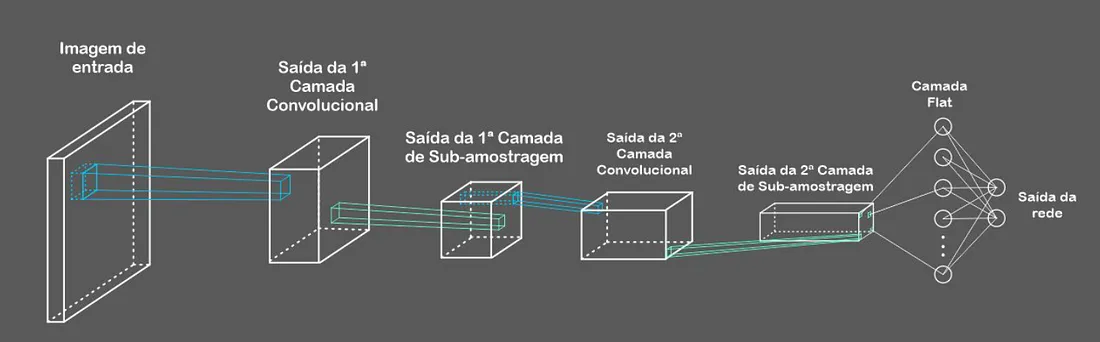
\includegraphics[width=1\linewidth]{cnn.png}
    \caption{Arquitetura de uma CNN.} \protect\href{https://vitorborbarodrigues.medium.com/conhecendo-a-vis%C3%A3o-do-computador-redes-neurais-convolucionais-e1c2b14bf426}{(\textcolor{blue}{Fonte})}
    \label{fig:cnn}
\end{figure}


\subsection{Componentes Técnicos}

\textbf{Fórmulas:}

\begin{equation}
(y * w)(i, j) = \sum_{m}\sum_{n} y(i+m, j+n) \cdot w(m, n)
\end{equation}

\begin{equation}
f(x) = \max(0, x)
\end{equation}

\begin{equation}
O = \left\lfloor \frac{n - f + 2p}{s} \right\rfloor + 1
\end{equation}

\begin{equation}
a^{[L]}_k = \frac{e^{z_k}}{\sum_{j=1}^{K} e^{z_j}}
\end{equation}

\subsection{Aplicação de CNN em Aplicativos de Namoro}

As Redes Neurais Convolucionais (CNNs) podem ser aplicadas eficazmente em aplicativos de namoro para entender e prever preferências visuais dos usuários, melhorando a experiência e personalização do serviço.

\begin{itemize}
    \item \textbf{Processamento de Dados de Imagem:}  
    Nos aplicativos de namoro, os usuários interagem com perfis, indicando suas preferências por meio de likes e dislikes. As CNNs podem ser treinadas para identificar padrões nas fotos dos perfis que recebem likes e dislikes, ajudando a determinar o que cada usuário considera atraente.

    \item \textbf{Treinamento da CNN:}  
    Um conjunto de dados grande e diversificado de imagens de perfis e interações de usuários é utilizado. A rede aprende a associar características visuais específicas com a probabilidade de um perfil receber um like.

    \item \textbf{Personalização de Recomendações:}  
    Uma vez treinada, a CNN pode ser integrada ao sistema de recomendação do aplicativo. Quando um novo perfil é apresentado, a CNN avalia as características visuais da imagem e prevê a probabilidade de um like com base nas preferências aprendidas.
\end{itemize}

Em resumo, a aplicação de CNNs em aplicativos de namoro é comum e muito eficaz como tecnologia de aprendizado profundo, potencializando o sucesso das interações e a eficácia de matches no aplicativo como um todo.


\section{Transformers}

\subsection{Introdução ao Conceito}
\textbf{}

\textbf{Definição:}  
Transformers são uma arquitetura de rede neural projetada para processar dados sequenciais de forma eficiente, utilizando o mecanismo de autoatenção. Introduzidos em 2017, os transformers superaram as redes recorrentes (RNNs) e as redes LSTM em diversas tarefas, especialmente no processamento de linguagem natural (NLP).

\textbf{Contextualização:}  
Transformers revolucionaram o campo do aprendizado profundo, particularmente em NLP, mas suas aplicações se expandiram rapidamente para outras áreas, incluindo visão computacional, processamento de áudio e aprendizado multi-modal. Sua capacidade de modelar dependências de longo alcance e capturar informações contextuais os tornaram o padrão ouro para a maioria das tarefas de NLP.

\subsection{Desenvolvimento Teórico}

\textbf{Explicação Detalhada:}

Os transformers são construídos com base em uma arquitetura de codificador-decodificador, que permite ao modelo analisar uma sequência de entrada, construir uma representação intermediária e, em seguida, gerar uma sequência de saída. Os principais componentes incluem:

\begin{itemize}
    \item \textbf{Mecanismo de Autoatenção:}  
    O mecanismo de autoatenção permite ao modelo pesar a importância de diferentes partes da sequência de entrada ao fazer previsões. Ele usa vetores de consulta, chave e valor para calcular scores de atenção, que determinam o foco em partes específicas da entrada.

    \begin{equation}
    \text{Attention}(Q, K, V) = \text{Softmax}\left(\frac{QK^T}{\sqrt{d_k}}\right)V
    \end{equation}

    Onde \(Q\), \(K\) e \(V\) são as matrizes de consulta, chave e valor, respectivamente, e \(d_k\) é a dimensão dos vetores de chave.

    \item \textbf{Codificadores e Decodificadores:}  
    O codificador transforma a entrada em uma representação de alto nível (vetor de contexto), enquanto o decodificador usa essa representação para gerar a saída.

    \item \textbf{Codificação Posicional:}  
    Como os transformers não possuem processamento sequencial inerente, eles utilizam codificações posicionais para injetar informações sobre a ordem dos tokens na sequência.

    \begin{equation}
    \text{PE}_{(pos, 2i)} = \sin\left(\frac{pos}{10000^{2i/d}}\right)
    \end{equation}
    \begin{equation}
    \text{PE}_{(pos, 2i+1)} = \cos\left(\frac{pos}{10000^{2i/d}}\right)
    \end{equation}

    Onde \(pos\) é a posição do token na sequência, \(i\) é o índice da dimensão, e \(d\) é a dimensão total dos embeddings.

    \item \textbf{Normalização de Camada e Conexões Residuais:}  
    A normalização de camada é usada para estabilizar e acelerar o treinamento. As conexões residuais ajudam na aprendizagem de redes profundas, mitigando problemas relacionados a gradientes desaparecendo.
\end{itemize}

\textbf{Fórmulas}

\begin{enumerate}
    \item \textbf{Autoatenção Escalonada:}  
    A autoatenção escalonada é calculada usando a seguinte fórmula, onde \(Q\), \(K\) e \(V\) representam as matrizes de consulta, chave e valor:

    \[
    \text{Attention}(Q, K, V) = \text{Softmax}\left(\frac{QK^T}{\sqrt{d_k}}\right)V
    \]

    Este mecanismo permite ao modelo identificar quais partes do texto são mais relevantes para cada parte da entrada.

    \item \textbf{Camadas de Normalização:}  
    A normalização de camada é aplicada para cada saída da camada, definindo a média e variância para estabilizar o treinamento:

    \[
    \text{LayerNorm}(x) = \frac{x - \mu}{\sqrt{\sigma^2 + \epsilon}}
    \]

    Onde \(\mu\) é a média e \(\sigma^2\) é a variância das ativações.
\end{enumerate}
\clearpage
  \begin{figure}
    \centering
    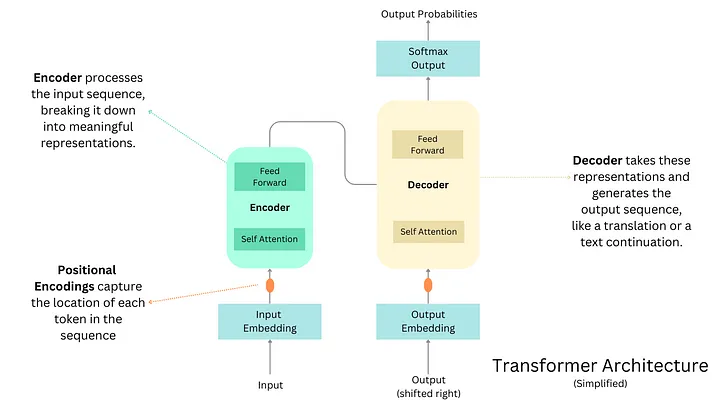
\includegraphics[width=0.8\linewidth]{transformer.png}
    \caption{Arquitetura de um Transformer.} \protect\href{https://medium.com/@tech-gumptions/transformer-architecture-simplified-3fb501d461c8}{(\textcolor{blue}{Fonte})}
    \label{fig:cnn}
\end{figure}
  \begin{figure}
    \centering
    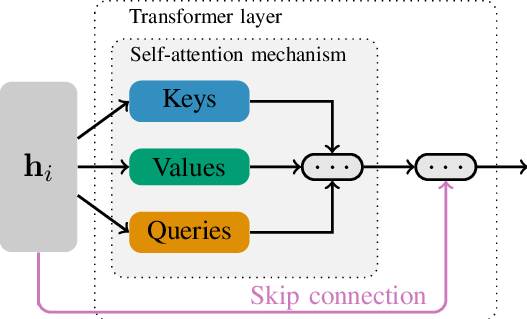
\includegraphics[width=0.4\linewidth]{selfattention.png}
    \caption{Mecanismo de Auto Atenção.} \protect\href{https://www.researchgate.net/figure/Simplified-computation-graph-for-the-i-th-layer-of-a-Transformer-Vaswani-et-al-2017_fig2_372163045}{(\textcolor{blue}{Fonte})}
    \label{fig:cnn}
\end{figure}



\subsection{Aplicação em Aplicativos de Namoro}

Transformers podem ser aplicados em aplicativos de namoro para aprimorar a análise de interesses e conexões sociais comuns entre usuários. Eles podem analisar descrições textuais, biografias de perfil e interações passadas para identificar interesses compartilhados e conexões sociais comuns, melhorando a qualidade das sugestões de matches.

\section{Redes Neurais de Grafos (GNNs)}

\subsection{Introdução ao Conceito}
\textbf{}

\textbf{Definição:}  
Redes Neurais de Grafos (GNNs) são uma classe de modelos de aprendizado profundo projetados para lidar com dados estruturados em grafos. Elas são capazes de capturar a topologia do grafo e aprender representações complexas de nós e arestas, aproveitando as relações intrínsecas e interações entre os componentes do grafo.

\textbf{Contextualização:}  
As GNNs têm sido amplamente adotadas em áreas como redes sociais, biologia computacional, sistemas de recomendação e processamento de linguagem natural, devido à sua capacidade de modelar dados não estruturados em um formato mais expressivo e relacional.

\subsection{Desenvolvimento Teórico}
\textbf{}

\textbf{Explicação Detalhada:}

As GNNs operam por meio da agregação de informações dos nós vizinhos, utilizando diferentes mecanismos de atualização e propagação de mensagens. Os principais componentes e operações incluem:

\begin{itemize}
    \item \textbf{Propagação de Mensagens:} 
    Este é o processo pelo qual cada nó coleta informações de seus vizinhos para atualizar sua própria representação. A propagação de mensagens permite que as GNNs capturem a estrutura local e as dependências de longo alcance no grafo.

    \begin{equation}
    \mathbf{h}_i^{(l+1)} = \text{AGGREGATE} \left(\left\{\mathbf{h}_j^{(l)}, \forall j \in \mathcal{N}(i)\right\}\right)
    \end{equation}

    \begin{equation}
    \mathbf{h}_i^{(l+1)} = \text{UPDATE} \left(\mathbf{h}_i^{(l)}, \mathbf{h}_i^{(l+1)}\right)
    \end{equation}

    Onde \(\mathcal{N}(i)\) representa o conjunto de vizinhos do nó \(i\), e as funções AGGREGATE e UPDATE são projetadas para combinar e atualizar as informações dos nós.

    \item \textbf{Normalização e Agregação:} 
    Métodos de normalização, como normalização simétrica, são usados para garantir que a contribuição de cada vizinho seja balanceada de acordo com o grau do nó. Isso promove uma propagação de informações mais consistente e robusta através do grafo.

    \item \textbf{Funções de Ativação e Pesos Treináveis:} 
    Funções de ativação, como ReLU, são aplicadas às representações agregadas, e pesos treináveis são usados para aprender as melhores transformações durante o processo de treinamento.
\end{itemize}

\clearpage
  \begin{figure}
    \centering
    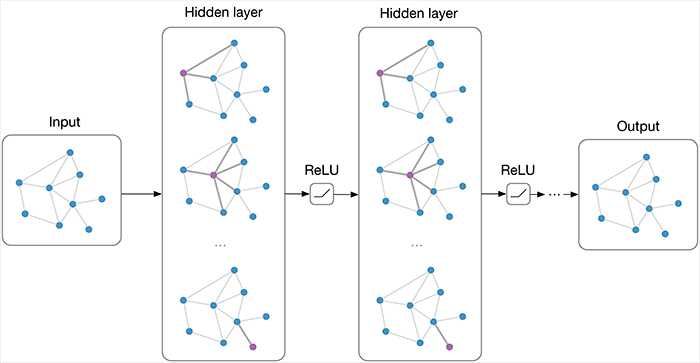
\includegraphics[width=0.8\linewidth]{image.png}
    \caption{Representação de uma GNN.} \protect\href{https://tkipf.github.io/graph-convolutional-networks/}{(\textcolor{blue}{Fonte})}
    \label{fig:cnn}
\end{figure}



\subsection{Componentes Técnicos}

\textbf{Fórmulas:}

1. \textbf{Propagação de Mensagens:}

\begin{equation}
\mathbf{h}_i^{(l+1)} = \sigma \left( \sum_{j \in \mathcal{N}(i)} \mathbf{W} \cdot \mathbf{h}_j^{(l)} + \mathbf{b} \right)
\end{equation}

Esta fórmula define a operação de uma camada em uma GNN, onde \(\mathbf{W}\) e \(\mathbf{b}\) são pesos treináveis, e \(\sigma\) é a função de ativação.

2. \textbf{Agregação com Normalização:}

\begin{equation}
\mathbf{h}_i^{(l+1)} = \sigma \left( \sum_{j \in \mathcal{N}(i)} \frac{1}{\sqrt{d_i d_j}} \mathbf{W} \cdot \mathbf{h}_j^{(l)} \right)
\end{equation}

Onde \(d_i\) e \(d_j\) são os graus dos nós \(i\) e \(j\), respectivamente.




\subsection{Conclusão}

As Redes Neurais de Grafos (GNNs) representam um avanço no aprendizado profundo, oferecendo um modo eficaz de modelar dados relacionais complexos. Em sistemas de recomendação para aplicativos de namoro, as GNNs podem ser utilizadas para explorar as interações e conexões sociais entre usuários. Ao modelar usuários e suas interações como nós e arestas, as GNNs conseguem identificar padrões de comportamento e compatibilidades baseadas não apenas em interesses comuns, mas também em influências sociais e interações passadas.

Essa abordagem pode aumentar a precisão das recomendações, ajudando a sugerir matches com maior potencial de sucesso e longevidade, oferecendo uma experiência de usuário mais personalizada e eficaz.
